\documentclass[a4paper,12pt]{book}

\setlength{\headheight}{1.1\baselineskip}
 
\usepackage[utf8]{inputenc}
\usepackage[spanish]{babel}

\usepackage{geometry}
\usepackage[sc]{mathpazo}

\usepackage{amsmath}

\usepackage[usenames,dvipsnames]{color} 
\usepackage{hyperref}
\usepackage{alltt}

% Para footer con páginas
\usepackage{scrpage2}
\usepackage{lastpage}

% Para insertar imágenes y ubicarlas
\usepackage{graphicx}
\usepackage{placeins}

% Para insertar código
\usepackage{xcolor}
\usepackage{listings}

\usepackage[T1]{fontenc} %%%key to get copy and paste for the code!

\usepackage{amssymb,amsmath}

% Source Code
\usepackage{color}
\usepackage{textcomp}
\usepackage{listings}
\usepackage{amsfonts}
\usepackage{courier}

\definecolor{source}{gray}{0.9}

% my comment style
\newcommand{\myCommentStyle}[1]{{\ttfamily\footnotesize\color{gray!100!white} #1}}

% my string style
\newcommand{\myStringStyle}[1]{{\ttfamily\footnotesize\color{violet!100!black} #1}}

% my symbol style
\newcommand{\mySymbolStyle}[1]{{\ttfamily\footnotesize\color{violet!100!black} #1}}

% my keyword style
\newcommand{\myKeywordStyle}[1]{{\ttfamily\footnotesize\color{green!70!black} #1}}

% my global style
\newcommand{\myGlobalStyle}[1]{{\ttfamily\footnotesize\color{blue!100!black} #1}}

% my number style
\newcommand{\myNumberStyle}[1]{{\ttfamily\footnotesize\color{brown!100!black} #1}}

\lstset{
language={},
% characters
tabsize=3,
escapechar={!},
keepspaces=true,
breaklines=true,
alsoletter={\#},
literate={\$}{{{\$}}}1,
breakautoindent=true,
columns=fullflexible,
showstringspaces=false,
% background
frame=single,
aboveskip=1em, % automatic space before
framerule=0pt,
basicstyle=\ttfamily\footnotesize\color{black},
keywordstyle=\myKeywordStyle,% keyword style
commentstyle=\myCommentStyle,% comment style
frame=single,%
backgroundcolor=\color{source},
% numbering
stepnumber=1,
numbersep=10pt,
numberstyle=\tiny,
numberfirstline=true,
% caption
captionpos=b,
% formatting (html)
moredelim=[is][\bfseries]{<b>}{</b>},
moredelim=[is][\textit]{<i>}{</i>},
moredelim=[is][\underbar]{<u>}{</u>},
moredelim=[is][\color{red}\uwave]{<wave>}{</wave>},
moredelim=[is][\color{red}\sout]{<del>}{</del>},
moredelim=[is][\color{blue}\underbar]{<ins>}{</ins>},
% smalltalk stuff
morecomment=[s][\myCommentStyle]{"}{"},
%    morecomment=[s][\myvs]{|}{|},
morestring=[b][\myStringStyle]',
moredelim=[is][]{<sel>}{</sel>},
moredelim=[is][]{<rcv>}{</rcv>},
moredelim=[is][\itshape]{<symb>}{</symb>},
moredelim=[is][\scshape]{<class>}{</class>},
morekeywords={true,false,nil,self,super,thisContext},
identifierstyle=\idstyle,
}

\makeatletter
\newcommand*\idstyle[1]{%
\expandafter\id@style\the\lst@token{#1}\relax%
}
\def\id@style#1#2\relax{%
\ifnum\pdfstrcmp{#1}{\#}=0%
% this is a symbol
\mySymbolStyle{\the\lst@token}%
\else%
\edef\tempa{\uccode`#1}%
\edef\tempb{`#1}%
\ifnum\tempa=\tempb%
% this is a global
\myGlobalStyle{\the\lst@token}%
\else%
\the\lst@token%
\fi%
\fi%
}
\makeatother


%\newcommand{\ct}{\lstinline[backgroundcolor=\color{white}]}
%\newcommand{\needlines}[1]{\Needspace{#1\baselineskip}}
\newcommand{\lct}{\texttt}

\lstnewenvironment{code}{%
    \lstset{%
    % frame=lines,
    frame=single,
    framerule=0pt,
    mathescape=false
    }%
    \noindent%
    \minipage{\linewidth}%
}{%
    \endminipage%
}%


\lstnewenvironment{codeWithLineNumbers}{%
    \lstset{%
    % frame=lines,
    frame=single,
    framerule=0pt,
    mathescape=false,
    numbers=left
    }%
    \noindent%
    \minipage{\linewidth}%
}{%
    \endminipage%
}%

%For simple inlined code
\newcommand{\ct}{\texttt}

%utiles e.g., i.e., c.f.
\usepackage{xspace}
\newcommand{\eg}{\emph{e.g.,}\xspace}
\newcommand{\ie}{\emph{i.e.,}\xspace}
\newcommand{\cf}{\emph{c.f.}\xspace}

%For comments
\usepackage{ifthen}
\newboolean{showcomments}
\setboolean{showcomments}{true}
\ifthenelse{\boolean{showcomments}}
  {\newcommand{\bnote}[2]{
	\fbox{\bfseries\sffamily\scriptsize#1}
    {\sf\small$\blacktriangleright$\textit{#2}$\blacktriangleleft$}
    % \marginpar{\fbox{\bfseries\sffamily#1}}
   }
   \newcommand{\cvsversion}{\emph{\scriptsize$-$Id: macros.tex,v 1.1.1.1 2007/02/28 13:43:36 bergel Exp $-$}}
	\newcommand{\del}[1]{\bnote{Remove}{\textcolor{gray} #1}}
  }
  {\newcommand{\bnote}[2]{}
   \newcommand{\cvsversion}{}
	\newcommand{\del}[1]{}
  } 

\newcommand{\gp}[1]{\bnote{Guille}{#1}}
\newcommand{\fd}[1]{\bnote{Fer}{#1}}

\newtheorem{definition}{Definición}

\newenvironment{codeNonSmalltalk}
{\begin{alltt}\ttfamily}
{\end{alltt}\normalsize}

% Para insertar boxes
\usepackage[framemethod=TikZ]{mdframed}
\mdfdefinestyle{BoxFrame}{%
    linecolor=black,
    outerlinewidth=1pt,
    roundcorner=20pt,
    innertopmargin=\baselineskip,
    innerbottommargin=\baselineskip,
    innerrightmargin=20pt,
    innerleftmargin=20pt,
    backgroundcolor=gray!30!white}

\renewcommand{\labelitemi}{$\bullet$}
\renewcommand{\labelitemii}{$\cdot$}
\renewcommand{\labelitemiii}{$\diamond$}
\renewcommand{\labelitemiv}{$\ast$}  

\ifoot[]{}
\cfoot{\thepage\ of \pageref{LastPage} }
\ofoot[]

\pagestyle{scrplain}

\vspace{0.1in}

\definecolor{dkgreen}{rgb}{0,0.6,0}
\definecolor{gray}{rgb}{0.5,0.5,0.5}
\definecolor{mauve}{rgb}{0.58,0,0.82}

\begin{document}

\chapter{Colecciones}
Las colecciones son un concepto importante y poderoso al diseñar con objetos. En este capítulo veremos cómo
se modela el conocimiento de un conjunto de referencias de un objeto y su utilización para resolver un problema
concreto.
\\
\\
Agradezco a Victoria Pocladova, Carlos Lombardi, Leonardo Volinier y Jorge Silva por el artículo 
``Colecciones en Smalltalk'' del sitio web \\
\begin{minipage}[t]{0.5\textwidth}
     \href{http://pdep.com.ar/material/apuntes}{{\color{blue}http://pdep.com.ar/material/apuntes}}
\end{minipage}
\\que en conjunto con el material que he preparado convergió en
el presente apunte.
\\
 \hfill Fernando Dodino

\tableofcontents

\section{Introducción}

\subsection{¿Qué es una colección?}
La colección nos permite representar un conjunto de objetos relacionados: los jugadores de un equipo de fútbol, 
un cardumen de peces, las cosas que un héroe guarda en su mochila, un ejército, son ejemplos de este
tipo de abstracciones.\\
\\
Otra definición posible es que una colección nos sirve para modelar una relación 1 a N:\\
\begin{itemize}
\item Una factura tiene muchas líneas con productos
\item Un escritor publicó varios libros
\item Una fiesta tiene muchos invitados
\item Un héroe tiene que cumplir varias misiones
\end{itemize}

A primera vista una colección es un conjunto de objetos. Si la vemos con más precisión nos damos cuenta que es más
preciso pensarla como un conjunto de referencias: los elementos no están adentro de la colección, sino que la
colección los conoce. 
\\
\\
\begin{figure}
    \centering
    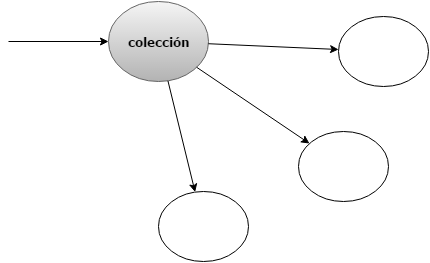
\includegraphics[width=0.8\textwidth]{images/01_GraficoInicial_Colecciones.png}
    \caption{La colección es un conjunto de referencias a otros objetos}
\end{figure}
\\
\subsection{Representación de colecciones}
Podemos graficar la relación dinámica entre un equipo de fútbol y los jugadores que lo integran mediante un diagrama
de objetos. Este es un diagrama con características \textit{dinámicas}, porque muestra el estado 
de los objetos en un momento determinado.
\\
\begin{figure}[h!]
    \centering
    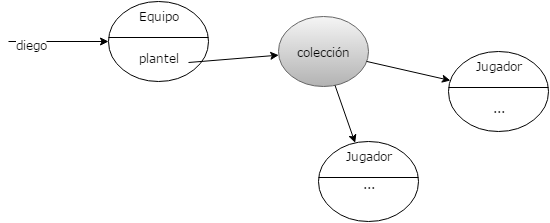
\includegraphics[width=0.9\textwidth]{images/02_Diagrama_Objetos_Equipo.png}
    \caption{El plantel de jugadores de un equipo como una colección de objetos}
\end{figure}
\FloatBarrier
También podemos generar un diagrama de clases en UML de la misma relación:
\begin{figure}[h!]
    \centering	
    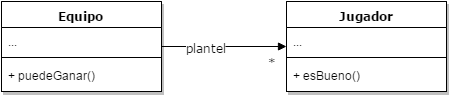
\includegraphics[width=0.9\textwidth]{images/03_Diagrama_Clases_Equipo.png}
    \caption{El plantel de jugadores, visto al nivel de clases}
\end{figure}
\FloatBarrier
Este es un diagrama con características \textit{estáticas}, porque no depende de un caso particular
sino que muestra las relaciones entre las clases.\\
\\
¿Qué es lo que cuenta el diagrama? Que un equipo \textbf{tiene} jugadores, el conector marca una relación
de \textbf{asociación}: hay un atributo plantel en la clase Equipo (el nombre del atributo se marca en uno
de los extremos de la asociación). El asterisco (*) muestra la multiplicidad: un equipo tiene muchos jugadores.
La dirección marca qué objeto conoce a los otros: como la flecha va de Equipo a Jugador sabemos que cada equipo
tiene n jugadores, no conocemos qué características tiene la relación de Jugador a Equipo, pero se pueden dar
dos opciones:
\begin{itemize}
\item un jugador pertenece a un solo equipo, en ese caso la relación Equipo-Jugador es de \textbf{uno a muchos}
\item un jugador participa en una relación con varios equipos (por ejemplo, porque nos interesa saber
en qué equipos jugó). En ese caso la relación es de \textbf{muchos a muchos}
\end{itemize}

\section{Interfaz de una colección}
Supongamos que tenemos un album de fotos, otra representación posible de una colección de objetos.
¿Qué podemos hacer con esas fotografías?
\\
\begin{itemize}
\item Mirarlas, ``recorrerlas'': iterar una colección
\item Averiguar cuántas fotos hay: saber su longitud
\item Saber si está una determinada foto en el album: saber si un elemento pertenece a la colección
\item Pegar una foto nueva: agregar un elemento a la colección
\item Regalar una foto a alguien: eliminar un elemento de la colección
\item Buscar qué fotos son de Ushuaia: filtrar/seleccionar elementos de una colección
\item Anotar las personas que salieron en mis fotos: transformar los elementos de una colección
\item Saber si hay alguna foto de Navidad: determinar si alguno/todos los elementos satisfacen 
un criterio
\end{itemize}
En el último requerimiento aparece también la idea de conjunto vacío. 
En general podemos asociar la noción matemática de conjunto a la colección, aunque sabemos que el conjunto
matemático no tiene orden, ni se ``recorre'', mientras que en la colección eso depende de la intención que
nosotros tengamos, como veremos más adelante.
\\
\section{Un ejemplo concreto}
En ciertos casilleros el héroe puede encontrar misiones y nuevos objetivos. Por ejemplo, un mago puede
encargarle buscar un ítem mágico en una montaña lejana. Un anciano puede encargarle liberar a su hija de
los terribles trolls que habitan en la gruta de los sin nariz. Cada vez que un héroe tiene uno de estos
encuentros, él anota los datos de la misión en su diario personal. Cada vez que una misión es superada,
el héroe la marca como “cumplida”. Toda misión suma en el camino del héroe: las misiones tienen una
recompensa de oro, y de respeto.
\\
\\
¿Qué abstracciones surgen? El héroe ahora tiene una colección de misiones. En principio vamos a pensar en
dos tipos de misiones: 1) buscar un ítem mágico, 2) liberar a una doncella. Las misiones deben tener una
recompensa (más adelante podemos modelar unidades de oro o de respeto para ello), un solicitante y el estado,
que puede ser pendiente o cumplida. Además nos avisan que existen misiones difíciles, que son
aquellas en las que el encargado es un ser justo, y además
\begin{itemize}
 \item si la montaña donde está el ítem a buscar queda a más de 100 kms. o bien 
 \item si la doncella a liberar está custodiada por más de 4 trolls
\end{itemize}

\subsection{Clases a crear - versión 0}
Vamos a crear lo mínimo necesario para poder meternos de lleno en el ejemplo de las colecciones.
Ahora el héroe tendrá una colección de misiones:

\begin{lstlisting}[frame=single]
Object subclass: #Heroe
	instanceVariableNames: 'misiones ...'
\end{lstlisting}

También vamos a crear una misión posible: BuscarItemMagico, por el momento sin atributos, porque nos queremos
seguir concentrando en la interfaz y no en la implementación, es decir, qué me ofrece el objeto y no cómo lo
resuelve.

Para poder agregar una misión, vamos a definir un método explícito:

\begin{code}
#Heroe
agregarMision: unaMision
  misiones add: unaMision
\end{code}

\subsection{Iniciamos un Playground}
Abrimos un Workspace de trabajo y vamos a inicializar un juego de variables nuevo:

\begin{code}
diego := Heroe new
  agregarMision: (BuscarItemMagico new)
\end{code}

Al intentar enviar el mensaje agregarMision: a diego se produce este error

\begin{figure}[h!]
    \centering	
    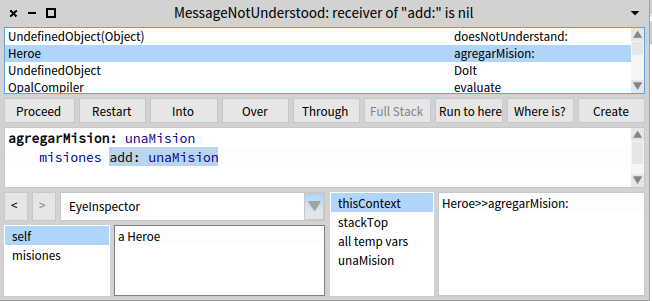
\includegraphics[width=0.9\textwidth]{images/11_error_agregarMision.png}
    \caption{La pantalla de \textit{debugging} muestra que el error ocurre al enviar el mensaje add: a misiones}
\end{figure}
\FloatBarrier

Esto se da porque la referencia a misiones quedó en nil. 

\begin{figure}[h!]
    \centering	
    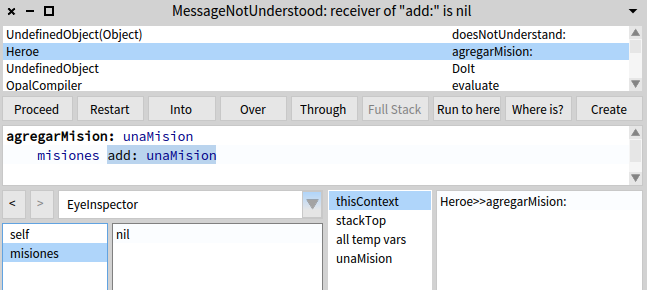
\includegraphics[width=0.9\textwidth]{images/12_error_debugging_2.png}
    \caption{misiones es una referencia a nil, ¡falta inicializarla!}
\end{figure}
\FloatBarrier

Entonces debemos inicializar a diego cuando creemos el guerrero, esto lo podemos hacer manualmente o con la opción
Analyze \textgreater Generate initialize method

\begin{figure}[h!]
    \centering	
    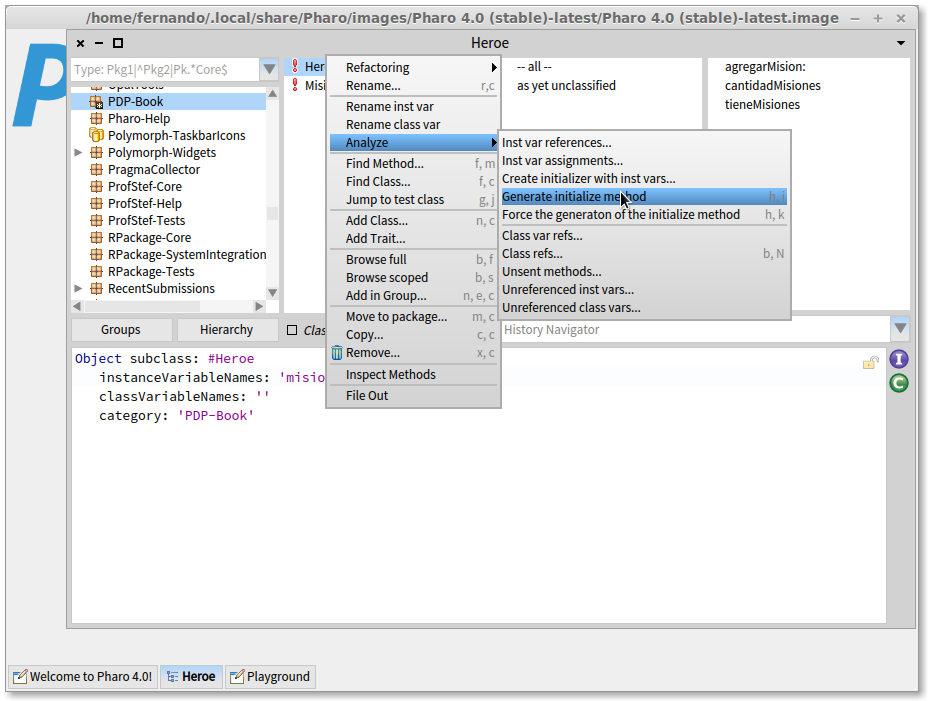
\includegraphics[width=0.9\textwidth]{images/13_generate_initialize.png}
    \caption{Generando un método initialize a través del IDE}
\end{figure}
\FloatBarrier

Comenzaremos usando un Set como colección, esto presupone que no nos importa el orden en el que almacenamos las
misiones y que no hay elementos duplicados: puede haber muchas liberaciones de doncellas, pero cada una 
representa una misión distinta. El Set es la implementación más equivalente al concepto matemático de conjunto
que presentamos anteriormente.
\\
Ahora sí nuestro método nos queda

\begin{code}
#Heroe
initialize
	super initialize.
	misiones := Set new.
\end{code}

y al grabarlo volvemos al Playground y ejecutamos nuevamente el código mediante Do It

\begin{code}
diego := Heroe new
  agregarMision: (BuscarItemMagico new)
\end{code}

vemos que el mensaje tuvo efecto inspeccionando la referencia diego: escribimos diego y luego Inspect It:

\begin{figure}[h!]
    \centering	
    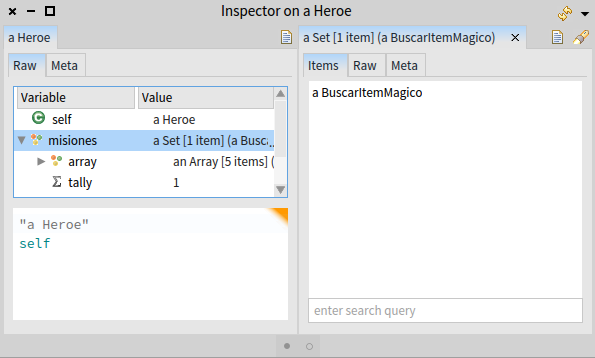
\includegraphics[width=0.9\textwidth]{images/14_coleccion_inicial.png}
    \caption{diego es un héroe y tiene una referencia en la colección misiones}
\end{figure}
\FloatBarrier


\subsection{Conocer el tamaño}
¿Cómo sabemos cuántas misiones tiene un héroe?

\begin{lstlisting}[frame=single]
#Heroe
cantidadMisiones
    ^misiones size
\end{lstlisting}
Y lo probamos, sabiendo que nos importa lo que va a devolver porque no es un método que tenga efecto, sino que
devuelve información, entonces elegimos la opción \textit{Print It}:

\begin{figure}[h!]
    \centering	
    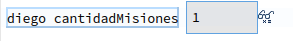
\includegraphics[width=0.6\textwidth]{images/15_diego_cantidadMisiones.png}
    \caption{diego tiene por el momento una sola misión}
\end{figure}
\FloatBarrier

\subsection{Saber si tiene elementos}
Queremos saber si un héroe tiene misiones...

\begin{lstlisting}[frame=single]
// Heroe
// Opcion 1
tieneMisiones
    ^misiones notEmpty
\end{lstlisting}

    
\begin{lstlisting}[frame=single]
// Opcion 2
tieneMisiones
    ^misiones size > 0
\end{lstlisting}

Ambas opciones parecen similares, de todas maneras la primera opción es más \textit{expresiva}. En la segunda
opción hay una traducción implícita: size \textgreater  0.... ah, es si tiene elementos. Es un detalle, pero un detalle que
implica tiempo que se pierde cada vez que vaya a leer la implementación de este método.

Lo probamos...
\begin{lstlisting}[frame=single]
diego tieneMisiones
\end{lstlisting}

\subsection{Clases a crear - versión 1}
Creamos la clase Mision, con atributos solicitante, recompensa y fecha de cumplimiento. Para cada uno de ellos 
definiremos los accessors correspondientes, haciendo botón derecho sobre la clase Mision > Refactoring > 
Inst Var Refactoring > Accessors 
\begin{figure}[h!]
    \centering
    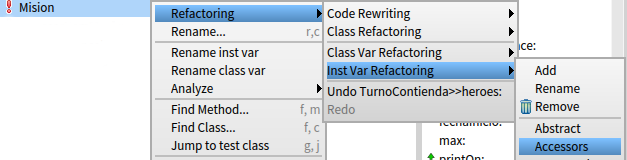
\includegraphics[width=0.9\textwidth]{images/10_accessors.png}
    \caption{El plantel de jugadores de un equipo como una colección de objetos}
\end{figure}
Dos subclases heredarán de Mision: 
\begin{itemize}
 \item BuscarItemMagico, necesitamos el atributo distanciaMontania
 \item LiberarDoncella, del cual necesitamos el atributo trollsSeguridad
\end{itemize}

* Interfaz de las colecciones siguiendo el ejemplo
  * Conocer el tamaño
  * Agregar un elemento
  * Sacar un elemento
  * Saber si tiene elementos
  * Buscar un elemento
  * Filtrar elementos que cumplan un criterio
  * Transformar los elementos de una colección generando otra colección
  * Totalizar valores que almacenan objetos de una colección, reducir una colección a un valores
  * Operatorias con conjuntos: includes/contains, union, intersection.
  * Saber si todos/algún elemento cumple una condición
  * Bloque de código y Declaratividad
* Iteradores externos e internos
* Tipos de colecciones. Estáticas vs. dinámicas. Ordenadas y sin ordenar. Con índices.
  Colecciones estáticas (Ejemplos de cada una de ellas. Formas de agregar elementos.)
  * Array
  * String
  * Interval
  
  Colecciones dinámicas
  * Bag?
  * Set
  * List/Ordered Collection
  * SortedCollection
  * Map/Dictionary
  * Comparativa general

  
  
\end{document}
